\documentclass[11pt]{article}
\usepackage{graphicx}
\usepackage{caption}
\usepackage{chngcntr}
\usepackage[section]{placeins} % subsections
\usepackage[round, sort, numbers]{natbib}
\usepackage{makecell}
\usepackage{url}
\counterwithin{figure}{section}
\captionsetup[figure]{slc=off}
\usepackage[left=2cm, right=2cm, top=2cm, bottom=2cm]{geometry} % geometry of page
\setcitestyle{square} % square referencing style
\usepackage[fleqn]{amsmath} % for maths
\usepackage{subfig}
\setlength{\parindent}{0pt} % no indents on new paragraphs
\graphicspath{{Code/Analysis/Figures/}}

\newcommand*\ruleline[1]{\par\noindent\raisebox{.8ex}{\makebox[\linewidth]{\hrulefill\hspace{1ex}\raisebox{-.8ex}{#1}\hspace{1ex}\hrulefill}}}

\begin{document}
\begin{titlepage}

    \begin{center}
        \vspace*{1cm}
        \Huge
        \textbf{Robotics} \\
        \vspace{0.5cm}
        \LARGE
        \vspace{1.5cm}
        \textbf{K. Mogilner, H. Tucker, T. Brent, A. Nicholls, G. Sheppard, D. Thomas, J. Doering, J. Matthews, C. Li} \\
        \vfill
        \vspace{0.8cm}
        \Large
        University of Birmingham\\
        Physics and Astronomy Department\\
    \end{center}
\end{titlepage}

\tableofcontents

\section{Abstract}
Wow look at \ref{angleplot}. \cite{Bae2006}.

\section{Introduction}
\subsection{Background}
\subsection{Motivation}
\subsection{Theory}

\section{Connecting}
\subsection{NAO}
David: you know what to write
also david write about how you sped up NAO's kicks somewhere it's juicy and tasty info
\subsection{Hinge Encoders}
George: difficulties for connecting on own computer, procedure for connecting on lab pc, need for libraries in right place etc, link to wiki in appendix

\section{Creating Algorithms}

\ruleline{George Sheppard}

The creation of each individual algorithm required a substantial amount of common code, for example: connecting to NAO, collecting angle values from both sets of hinge encoders, and processing these data. For this reason the code was structured such that new algorithms could be freely created that each integrated with the base code. This base code collected all values relating to the swinging motion, passed these values through an algorithm, stored these values, and fixed the cycle rate. Additionally, due to this structure, mock classes for NAO and the hinge encoders were created such that this interface could be developed away from the lab, and a testing setup was added such that a user would be able to re-run previous recorded data and plot how their algorithm reacted to that scenario.\\

With this base structure in place, creating an algorithm involved one function that took a set of values, and decided how to react to them, the algorithm also had access to all past data to help in decision making. As these algorithms were defined in the same way, it is easy to switch between different algorithms mid swing, such that the motion of NAO could be more stringently controlled. For example NAO could be told to increase to $30^o$, then maintain this amplitude for $10s$, and then finally decrease back down to $0^o$.  This base structure also included the pre-defined positions for NAO, such that switching positions could be done by just calling a function with the name of the position.

\section{Simple Pendulum}
\subsection{Start Up}

\ruleline{James Doering}

\textit{James: talk about two positions defined for the motion, idea behind the algorithm, how it links into the next algorithm that increases amplitude, results, why is it tricky to start off like this (have to predict when to swing very well sort of stuff), if multiple algorithms created do for each} \\

There are multiple tactics for beginning a swing from rest - the most intuitive is to "kick off" from an object to give an initial amplitude, which a human would achieve by pushing themselves from the floor. This method was approached by previous years by creating a box for the robot to push away, or by manually giving it an intial amplitude. This was further developed upon by giving the robot a method of starting with zero assistance. By utilising the angular velocity gained by the swing when the robot's legs swing (as described in section INSERT REF). \\

For the start-up algorithm, very little input is required - the motion is effectively pre-calculated, as the initial conditions are the same each time, with NAO starting from rest. Parametric motion cannot be used to start the swing, and so changes in angular momentum of NAO's legs must be used instead. To achieve this, two postures were defined: 'seated', with the legs tucked beneath the seat and the chest pulled in to the bar, and 'extended', with the legs extended out and the chest pushed away from the bar. These two postures can be seen in figure \ref{fig:seatedextended}.\\

    \begin{figure}
        \centering
        \includegraphics{}
        \caption{The 'seated' and 'extended' positions used in the start-up script and TORQUE method.}
        \label{fig:seatedextended}
    \end{figure}

The algorithm is very simple - an initial kick is made, going from the seated to the extended posture, which in turn gives the swing some small angular momentum. The robot does not move until a quarter-period has passes, when it should be at the peak of its backward swing. It then kicks into the seated position, and waits for a half period so it is at its next peak, before switching postures again. This loop of waiting a half-period and kicking is repeated until a minimum amplitude is reached (1 degree), where it then switches to another algorithm. This was done smoothly by only switching after a short time had passed since its last kick, preventing the next algorithm from immediately calling for a new kick.\\

This start-up was made even more effective by adding extra weight to the robot's feet, and so increasing the angular momentum produced in the swing - the difference in motion of the two methods can be seen in figure \ref{fig:startupcomparison}. This helped counteract the large mass of the swing and the small mass of NAO.


    \begin{figure}
        \centering
        \includegraphics{}
        \caption{A plot showing the difference in amplitude gained for the start-up script with the default robot and the robot with extra weight in its feet.}
        \label{fig:startupcomparison}
    \end{figure}



\subsection{Increasing and Decreasing Amplitude}
\subsubsection{Parametric Pumping}
Jon: Talk about two extra positions defined for this motion, the idea behind the algorithm, results try to fit to exponential curve to see if it multiplies amplitude by fixed fraction like worksheet showed, any limitations, were two positions just different in vertical centre of mass or did horizontal distance change too
\subsubsection{Torque Method TODO: BETTER NAME FOR THIS}
George/David: Say used previous defined positions, different methods for each algorithm (quarter period, theory team calculation of max angle), results for each, try to fit maximum amplitude peaks to linear to see if proportional to distance rocked or not, how results varied on different parameters such as if he swings before peak, during, or after, limitations to each method

\subsection{Maintaining Amplitude}
Chenglong: different subsubsection for each method you used, first outline the idea behind each algorithm, then show the results for each, compare and contrast after you have shown results for each, which was easiest to code, had the finest control over the angle (calculate variance on the maximum amplitude of the swing), which is most efficient, anything else you decide is good

\subsubsection{Conclusion}
Everyone: Think this should just be how to improve, any difficulties of the setup, which is the best method and why etc

\section{Triple Pendulum}

    \begin{figure}[!htb]
        \centering
        \captionbox
             {Angleplot.\label{angleplot}}
             {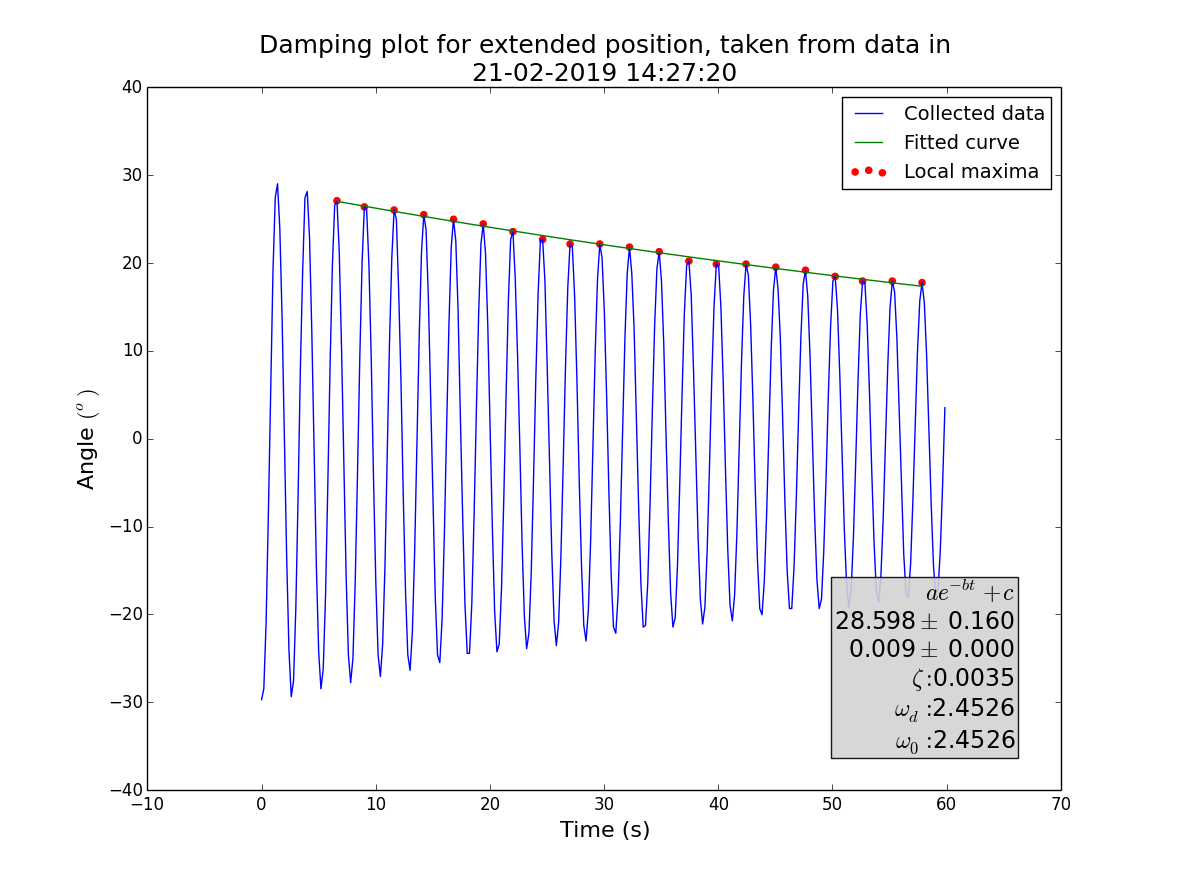
\includegraphics[width=1.0\textwidth]{ExtendedPositionDamping.png}}}
    \end{figure}

\subsection{Start Up}
\textit{We will probably just copy the code straight over so just say that.}


\appendix
\section{Appendix}
\subsection{Wiki} \label{sec:wiki}
\ruleline{George Sheppard}
Throughout this project, there were a large amount of issues found when trying to connect to: NAO, Webots, and the hinge encoders etc. For this reason a wiki was created to document how to set everything up correctly. This wiki is available at: https://github.com/GeorgeSheppard/Robotics. Alongside this wiki is the final code, including how to use it, the report, and any analysis files used to create plots. Feel free to clone this repository and add to it such that there remains a comprehensive guide for each year.

\subsection{Webots}
\ruleline{James Doering}
Webots offers a substantial amount of uses - throughout this project Webots was used to test the interface and algorithms away from the lab, and to find accurate estimates for NAO's centre of mass in different positions. However, Webots did not offer much in useful physical simulations - the simulated swing would often fail, and physics would quickly go out of sync if the target frame-rate was missed momentarily. In order to interface with Webots from the NAOQI python library (supplied by Aldebaran/SoftBanks), the NAOQISIM controller was required - this acted as a 'virtual robot' to translate from Python script written with NAOQI to the NAOQISIM controller in Webots, which controlled the simulated NAO. This proved difficult to achieve, only being possible with certain software configurations. It is highly recommended that this is done on a linux operating system, otherwise there will be errors between 32 and 64 bit versions of python and NAOQI/NAOQISIM. The version of NAOQI required to connect to Webots is different to the version required to connect to the real NAO - as of writing, Webots/NAOQISIM requires NAOQI 2.1.4.13, whereas NAO requires NAOQI 1.14.5. Further explanation can be seen on the wiki decribed in section \ref{sec:wiki}.

\bibliographystyle{ieeetr}
\bibliography{References}
\end{document}